\documentclass[border=10pt]{standalone}
\usepackage{tikz}\usepackage{amsmath}\usetikzlibrary{arrows.meta,decorations.markings}
\begin{document}
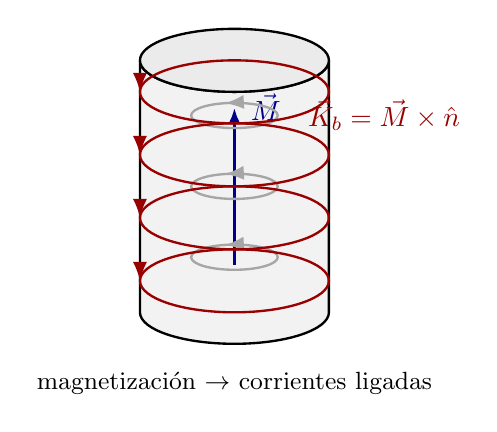
\begin{tikzpicture}[line width=0.85pt,>={Latex[length=2mm]}]
  % cilindro 3D
  \draw[fill=black!5] (-1.2,-1.6) -- (-1.2,1.6) arc (180:360:1.2 and 0.4) -- (1.2,-1.6) arc (0:-180:1.2 and 0.4);
  \draw[fill=black!8] (0,1.6) ellipse (1.2 and 0.4);
  % M axial
  \draw[->,blue!55!black,line width=1.3pt] (0,-1.0)--(0,1.0) node[right=2pt]{$\vec M$};
  % loops internos (cancelan)
  \foreach \y in {-0.9,0,0.9} \draw[gray!70,decoration={markings,mark=at position 0.3 with {\arrow{Latex}}},postaction={decorate}] (0,\y) ellipse (0.55 and 0.16);
  % corriente ligada superficial K_b
  \foreach \y in {-1.2,-0.4,0.4,1.2} \draw[red!60!black,decoration={markings,mark=at position 0.5 with {\arrow{Latex}}},postaction={decorate}] (0,\y) ellipse (1.2 and 0.4);
  \node[red!60!black] at (1.9,0.9){$\vec K_b=\vec M\times\hat n$};
  \node at (0,-2.5){\small magnetización $\to$ corrientes ligadas};
\end{tikzpicture}
\end{document}
